\documentclass[conference]{configs/IEEEtran}
\IEEEoverridecommandlockouts
% The preceding line is only needed to identify funding in the first footnote. If that is unneeded, please comment it out.
\usepackage{cite}
\usepackage{amsmath,amssymb,amsfonts}
\usepackage{algorithmic}
\usepackage{graphicx}
\usepackage{textcomp}
\usepackage{xcolor}
\usepackage{hyperref}
%\usepackage[table,xcdraw]{xcolor}
\def\BibTeX{{\rm B\kern-.05em{\sc i\kern-.025em b}\kern-.08em
    T\kern-.1667em\lower.7ex\hbox{E}\kern-.125emX}}
\begin{document}

\title{Development of Performance Regression Analysis Tool using Distributed Tracing on Microservice-based Application\\
%{\footnotesize \textsuperscript{*}Note: Sub-titles are not captured in Xplore and should not be used}
%\thanks{Identify applicable funding agency here. If none, delete this.}
}

\author{\IEEEauthorblockN{Rafi Abbel Mohammad}
\IEEEauthorblockA{\textit{School of Electrical Engineering and Informatics} \\
\textit{Institut Teknologi Bandung}\\
Bandung, Indonesia \\
masterraf21@gmail.com}
%\and
%\IEEEauthorblockN{Achmad Imam Kistijantoro}
%\IEEEauthorblockA{\textit{School of Electrical Engineering and Informatics} \\
%\textit{ITB, Indonesia}\\
%Bandung, Indonesia \\
%imam@stei.itb.ac.id}
}

\maketitle

\begin{abstract}
In applications with Microservice architecture, when a significant change occurs and result in decreased performance or regression, it is difficult to perform analysis to check which part of the whole Microservice is the main cause of the regression due to the distributed nature of Microservice. Distributed tracing can be used to analyze and determine whether there is a regression and the cause of the regression by utilizing latency data from existing operations on Microservice application.
This system will perform performance regression analysis using the distributed tracing tool Zipkin. Regression is then can be detected using Kolmogorov-Smirnov statistical analysis which will compare the latency data samples that occur
periodically and the sample latency baseline data that represents application performance  under normal circumstances. The analysis will compare the Cummulative
Distribution Function (CDF) of the two samples and see if both
CDF comes from a different distribution. If it is found that both CDFs originate from different distributions, it then can be suspected that there has been a performance regression because the distribution of the periodic data has deviated from the distribution of the baseline data.
If a regression is detected, the system will then perform a critical path analysis to see which operations of each services are most likely contributed to the regression. The analysis will be carried out by finding the difference
latency of periodic and baseline operation data and it will be seen which operation's latency difference exceeds a predetermined limit.
The performance regression analysis system has been tested on a Microservice application that runs on Kubernetes. The result is that out of 10 out of 11 test cases, and for every successful case, the main suspected operation that causes regression is found. Implementing the system adds an average overhead of 0.78\% CPU usage and 0.67\% Memory usage.
\end{abstract}

\begin{IEEEkeywords}
performance regression, Distributed Tracing, Microservice, Kubernetes
\end{IEEEkeywords}

\section{Introduction}
\label{1}
With the widespread adoption use of Microservice architecture based on distributed systems today, more and more challenges arise related to the adoption of this architectural style. Microservice architecture offers several advantages, including technological heterogeneity, resilience, ease of \textit{scaling}, ease of \textit{deployment}, ease of alignment with a technology team, flexibility in determining application composition, and an optimized system to replace components with each other \cite{building-microservices}. These advantages make the adoption of the Microservice architecture quite widespread, especially in applications that require \textit{scalability} to serve the growing needs of customers.

However, with the many advantages offered by the Microservice architecture, it will also increase the complexity to perform analysis when there is a decline in performance or regression in the application. This is due to the distributed nature of Microservice by dividing the application into smaller services, so to find which operation of the services causing the regression will be difficult and will be inefficient to perform analysis on each and every available services, especially if the number of the services has reached hundreds or thousands.

There is already a tool that can help developers to perform monitoring on distributed systems such as Microservice, which is distributed tracing. With the help of trace, developers can get an overview of each request that occurs in a resource or component that interacts with other components in a distributed system such as node, service, network, or mutex. The traces then can be processed for various purposes, such as creating a dependency map between services, perform a performance analysis of the service, and also perform a performance regression analysis using the latency data from the trace result.

We provide the implementation of the performance regression analysis (PRA) system using the distributed tracing tool Zipkin which is available on Github\footnote{\url{https://github.com/masterraf21/pra\textunderscore engine}}. The PRA system will perform detection on the Microservice application when a regression occurs and perform analysis to determine the main cause of the regression. Performance regression analysis will be done by using the help of the trace results from Zipkin which will be able to help developers restore performance of Microservice application after reggresion occurs.

The paper is organized as follows. Section II presents related
work in the area of performance regression and distributed tracing. Section III discusses problem analysis, the design and the underlying architecture, and the implementation of the PRA system. Section IV shows the experiments done with the PRA system. Section V discusses a few analysis from the experiments done in Section V. Section
VI concludes the work.


\section{Related Works}

\section{Proposed Solution}
This section explains analysis of the problem introduced in section \ref{1}, the general solution to solve the problem, the architecture, and the implementation of the system.

\subsection{Problem Analysis}
As the complexity of Microservice applications increases, such as with the increasing number of servce and the connectivity between existing servces therein, there will also be an increase in the complexity of monitoring the performance on the entire Microservice application. One of the important issues related to performance is a regression or decrease in performance. The need for urgently determining the main cause of the regression in the system becomes important if the regression occurs in a production environment that directly serves requests from customers, so that if it is not addressed immediately it will have a direct impact on the
user experience in using the application.

There are two approaches that can be taken to solve the problem of performance regression \cite{regression-detection}, namely:
\begin{enumerate}
	\item Regression detection is carried out after the application has been developed and deployed in a dedicated environment:
	\item Regression detection is carried out before the application is developed and deployed, and then conducting a study of the resulting changes to the source code
\end{enumerate} 

Given the distributed nature of Microservices, it will be difficult for developers if regression detection is carried out with an individual approach on each existing servce especially when the number of existing servce is very large, and the interdependence relationship between services becomes complicated. Therefore, to overcome performance regression in Microservice-based application, an approach that does not require developers to source search is needed. So that in the case of detection and regression analysis of Microservice-based application performance, the first approach is more suitable to use.

Therefore, the workflow that must be carried out by the performance regression analysis (PRA) system is as follows:
\begin{enumerate}
	\item The system must be able to detect when there is a regression in Microservice-based application
	\item The system must be able to determine the source or root cause of the regression after it is detected
\end{enumerate}

Seeing the needs of the PRA system above, the approach the will be carried out to do performance regression analysis will be Cummulative Analysis and Aggregation Analysis. 

Cummulative Analysis is an approach to analyze certain metrics of application such as latency by cummulating all the collected data as a single representation such as Histogram. With this approach, the distributed nature of many services in Microservice-based application can be observed as a single figure or representation so that the whole Microservice application can be monitored in a single space. One of the available tool to analyze and compare large sets of data is called Kolmogorov-Smirnov (K-S) statistic test. The K-S statistic test will count the difference between two Cummulative Distribution Functions (CDF) as a scalar number \cite{kolmogorov_1951}.

K-S statistic are obtained by finding the furthest vertical distance between the two CDFs as indicated by the arrows. The greater the distance, the more likely it is that two CDFs are from two different distributions so that it can be an indication that there has been a change on performance.
\begin{figure}[htb]
	\centering
	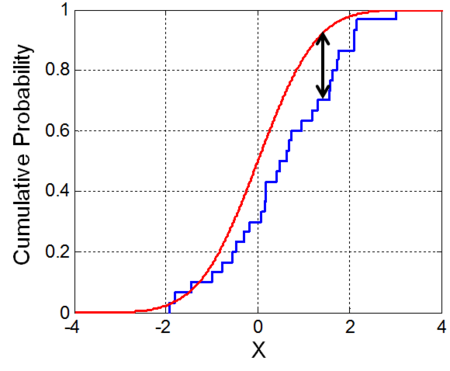
\includegraphics[width=0.35\textwidth]{resources/ch2/ks.png}
	\caption{CDF of two samples, arrows indicate the Kolmogorov-Smirnov statistical value \cite{wiki:ks-test}}
	\label{ks-example}
\end{figure}

The Cummulative Analysis approach will be used to fullfil the first needs of the PRA system by using Kolmogorov-Smirnov statistic test.

On the other hand, Aggregation Analysis can help to identify changes that are not too visible on the performance of a service. When comparing two sets of traces, we can also see the latency contribution associated with the tag,
operations, and services and also see how these contributions change over time time. Average contribution metric
such as the latency of each service and its operation will be determined from each set. Then the mean difference of the contribution metrics from the baseline and regression sets
will be calculated and sorted so that it can be seen which operation or service is actually the root cause of the regression.

Tab. \ref{aggregate} shows the result of the Aggregation Analysis approach which will be useful in determining the possible root cause of the regression. This approach will be used to fullfil the second needs of the PRA system.
\begin{table}[!htb]
	\caption{Aggregation Analysis result}
	\label{aggregate}
	\centering
	\begin{tabular}{|l|l|l|l|}
		\hline
		\textbf{Service/Operation} & \textbf{Baseline} & \textbf{Regression} & \textbf{Difference} \\ \hline
		inventory/write-cache & 63.1 ms & 368 ms  & +305 ms  \\ \hline
		inventory-db/update   & 1.75 ms & 2.26 ms & +0.51 ms \\ \hline
		memcached/set         & 4.94 ms & 4.71 ms & -0.23 ms \\ \hline
		inventory/update      & 15.2 ms & 14.8 ms & -0.47 ms \\ \hline
		inventory/db-update   & 32 ms   & 30.6 ms & -1.4 ms  \\ \hline
	\end{tabular}
\end{table}

Fig. \ref{flow-pra} illustrates the phases to be carried out by the PRA system. In general, there will be two phases to be carried out, namely the baseline loading phase
and the periodic analysis phase. The first phase, namely the loading phase, will look for stable application activity data that can be used as a baseline or a reference for the analysis to be carried out in the next stages. This phase
will produce two artifacts, the latency data of all recorded traces by the tracing system, and operating data that occurs on the critical path of all traces along with its latency value which will be stored as a key-value pair as well.
\begin{figure}[!htb]
	\centering
	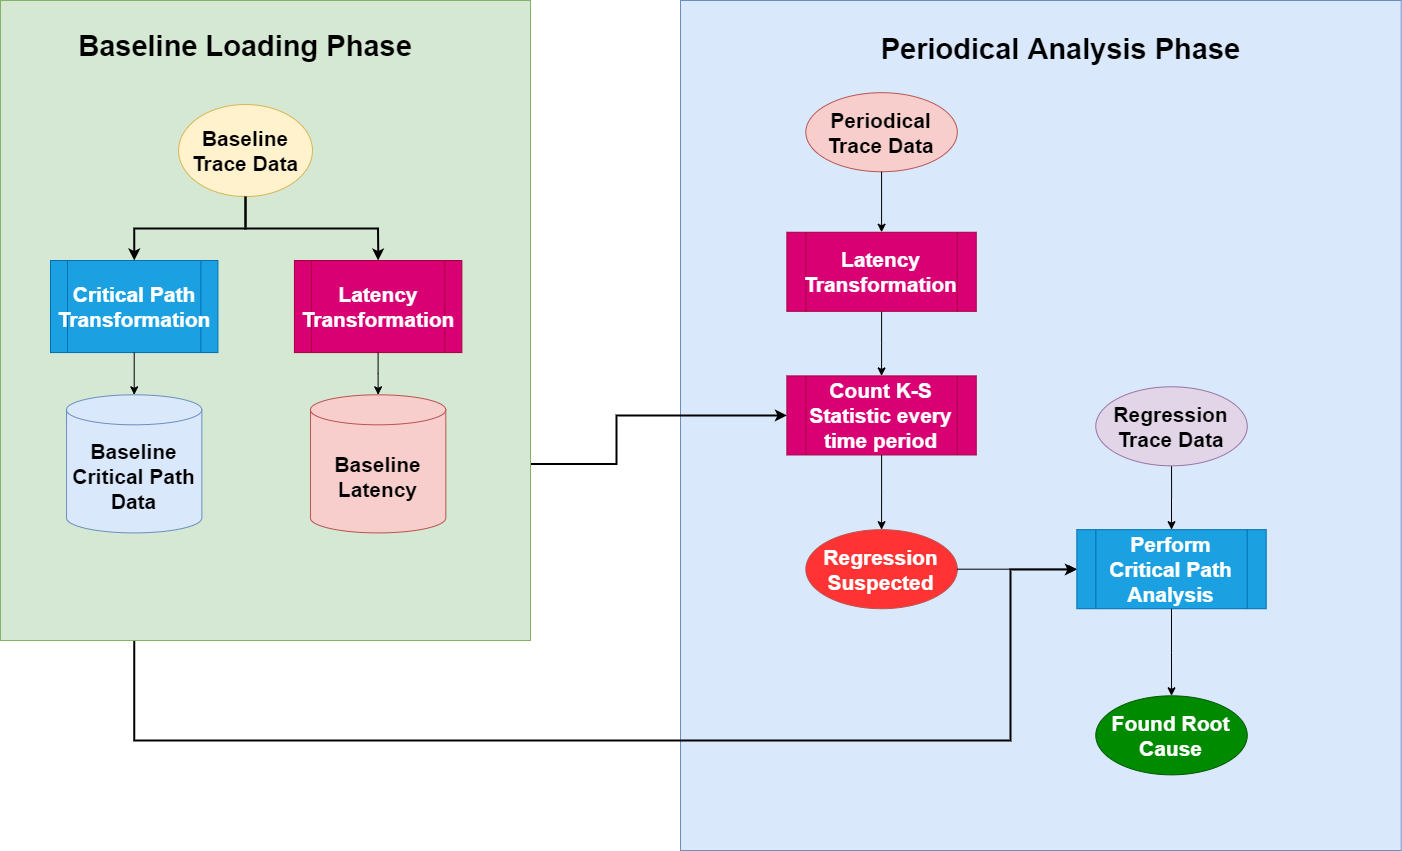
\includegraphics[width=0.5\textwidth,scale=5]{resources/ch3/alur_v2.png}
	\caption{PRA system workflow}
	\label{flow-pra}
\end{figure}

The next phase is the periodical analysis phase. This phase will run continuously and the analysis will be run periodically at intervals of every 5 minutes. This is carried out to continuously detect whether there is a regression and
immediately determine the source of the regression if it occurs. There are several stages of analysis
to be carried out in this phase. The first analysis stage will compare the results transformation of data latency of all ongoing traces periodically with the baseline latency artifact from the loading phase. The comparison will be made within a certain period. The comparison of the two latency data will produce Kolmogorov-Smirnov statistic. If the Kolmogorov-Smirnov statistic that is generated indicates that the two samples of latency data come from two different distributions, then it can be an indication that there has been a regression in the data capture in the periodical phase.

If a regression is detected, the next step is to perform a critical path analysis by calculating the contribution of the critical path data trace from the regression period and will be compared with the critical path data derived from the baseline calculation. From this comparison, it will be sorted and the result of which operation has the largest latency difference becomes strong candidate as the root cause of the regression.



\subsection{Architecture}
Fig. \ref{arch-pra} shows the architecture of the PRA system. There will be only two components that will be implemented from scratch, which are the PRA Engine and the PRA UI. The rest of the components are already present and ready to use from Zipkin. The PRA Engine will fetch data from Zipkin API to retrieve the traces generated and will implement the logic from Fig \ref{flow-pra}. The PRA Engine will be exposed as an Application Programming Interface (API). The PRA UI will fetch data from the PRA Engine API and will present the state of regression in the application, and the critical path analysis result.
\begin{figure}[!htb]
	\centering
	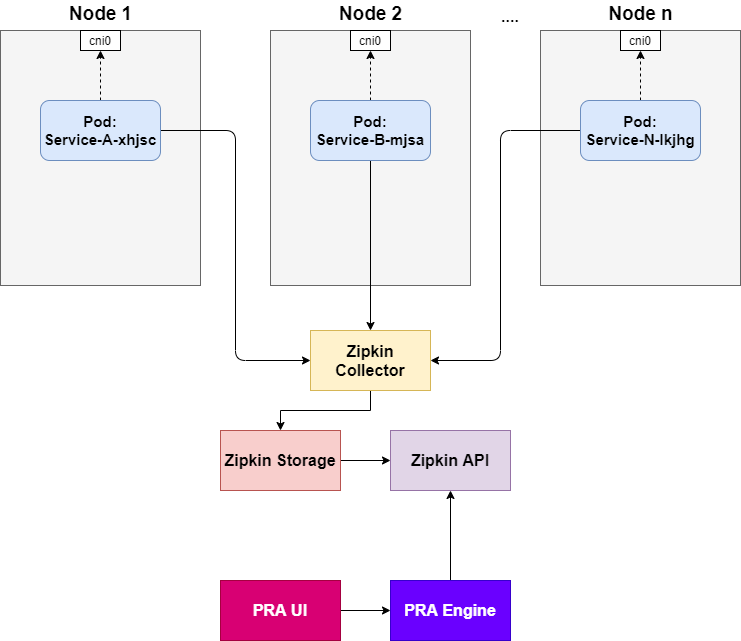
\includegraphics[width=0.4\textwidth]{resources/ch3/arch.png}
	\caption{PRA system architecture}
	\label{arch-pra}
\end{figure}

\subsection{Implementation}
Implementation of the performance regression analysis (PRA) system will be made based on the architectural design as shown in Fig. \ref{arch-pra}. Component
like the instrumentation library instead will use the available
Open Source distributed tracing from Zipkin. Components to be made from scratch entirely are the PRA User Interface (UI) and PRA Engine components of the system.

\subsubsection{PRA Engine Implementation}
Before implementing the solution, we  must first
select the tools that will be used to do the implementation. In general, there are many programming languages that can implement solutions of the PRA Engine. However, there is
an important need to implement the Kolmogorov-Smirnov (K-S) statistical test which not all programming languages have a support library to do this. There are two programming languages that have libraries for performing K-S tests
which are the Go and Python programming languages. The Go language has the Gonum\footnote{\url{gonum.org}} library which
has a K-S test implementation in the \texttt{KolmogorovSmirnov} function, while the language
Python has the SciPy\footnote{\url{scipy.org}} library which has a K-S test implementation in the \texttt{scipy.stat.ks\textunderscore 2samp} function.

\subsubsection{PRA UI Implementation}

\section{Experiment}

\section{Analysis}

\section{Conclusion \& Future Works}

%\section*{Acknowledgment}
%
%The preferred spelling of the word ``acknowledgment'' in America is without 
%an ``e'' after the ``g''. Avoid the stilted expression ``one of us (R. B. 
%G.) thanks $\ldots$''. Instead, try ``R. B. G. thanks$\ldots$''. Put sponsor 
%acknowledgments in the unnumbered footnote on the first page.

\bibliographystyle{configs/IEEEtran}
\bibliography{references}

\vspace{12pt}


\end{document}
